% Notes:
% - The point that central regions of low J_z, density flattens = no constraining power
% - The condition on d(r_z)/d(r_z')
% - Widmark papers
% - https://arxiv.org/abs/2303.18040


% TODO:
% - We don't actually need to bring in the CBE at all. Much simpler point about functions that are constant along an orbit.
% - cite Justin Read review, and https://arxiv.org/pdf/2012.11477.pdf


% \begin{figure}[!t]
% \begin{center}
% % \includegraphics[width=0.9\textwidth]{visitstats.pdf}
% {\color{red} Figure placeholder}
% \end{center}
% \caption{%
% TODO
% \label{fig:chiplots}
% }
% \end{figure}

\PassOptionsToPackage{usenames,dvipsnames}{xcolor}
% \documentclass[modern]{aastex631}
\documentclass[twocolumn]{aastex631}

% Load common packages
\usepackage{microtype}  % ALWAYS!
\usepackage{amsmath}
\usepackage{amsfonts}
\usepackage{amssymb}
\usepackage{booktabs}
\usepackage{graphicx}
% \usepackage{color}

\usepackage{enumitem}
\setlist[description]{style=unboxed}

% Some style hacks:
% \renewcommand{\twocolumngrid}{\onecolumngrid}
\setlength{\parindent}{1.1\baselineskip}
\addtolength{\topmargin}{-0.2in}
\addtolength{\textheight}{0.4in}
\sloppy\sloppypar\raggedbottom\frenchspacing

\graphicspath{{figures/}}
% \definecolor{cbblue}{HTML}{3182bd}
% \usepackage{hyperref}
% \definecolor{linkcolor}{rgb}{0.02,0.35,0.55}
% \definecolor{citecolor}{rgb}{0.45,0.45,0.45}
% \hypersetup{colorlinks=true,linkcolor=linkcolor,citecolor=citecolor,
%             filecolor=linkcolor,urlcolor=linkcolor}
% \hypersetup{pageanchor=true}

\newcommand{\documentname}{\textsl{Article}}
\newcommand{\sectionname}{Section}
\renewcommand{\figurename}{Figure}
\newcommand{\equationname}{Equation}
\renewcommand{\tablename}{Table}

% Missions
\newcommand{\project}[1]{\textsl{#1}}

% Packages / projects / programming
\newcommand{\package}[1]{\textsl{#1}}
\newcommand{\acronym}[1]{{\small{#1}}}
\newcommand{\github}{\package{GitHub}}
\newcommand{\python}{\package{Python}}
\newcommand{\jax}{\package{JAX}}
\newcommand{\emcee}{\project{emcee}}

% Stats / probability
\newcommand{\given}{\,|\,}
\newcommand{\norm}{\mathcal{N}}
\newcommand{\pdf}{\textsl{pdf}}

% Maths
\newcommand{\dd}{\mathrm{d}}
\newcommand{\deriv}[2]{\frac{\mathrm{d}{#1}}{\mathrm{d}{#2}}}
\newcommand{\dderiv}[2]{\frac{\mathrm{d^2}{#1}}{\mathrm{d}{#2}^2}}
\newcommand{\Deriv}[2]{\frac{\mathrm{D}{#1}}{\mathrm{D}{#2}}}
\newcommand{\pderiv}[2]{\frac{\partial {#1}}{\partial {#2}}}
\newcommand{\ppderiv}[2]{\frac{\partial^2 {#1}}{\partial {#2}^2}}
\newcommand{\transpose}[1]{{#1}^{\mathsf{T}}}
\newcommand{\inverse}[1]{{#1}^{-1}}
\newcommand{\argmin}{\operatornamewithlimits{argmin}}
\newcommand{\mean}[1]{\left< #1 \right>}

% Non-scalar variables
\renewcommand{\vec}[1]{\ensuremath{\bs{#1}}}
\newcommand{\mat}[1]{\ensuremath{\mathbf{#1}}}

% Units:
% Workaround for siunitx + AASTeX
% https://tex.stackexchange.com/questions/192610/use-emulateapj-aastex-with-siunitx
\usepackage{savesym}
\savesymbol{tablenum}
\usepackage{siunitx}
\restoresymbol{SIX}{tablenum}
\DeclareSIUnit\year{yr}
\DeclareSIUnit\parsec{pc}
\DeclareSIUnit\Msun{M_\odot}
\DeclareSIUnit\Rsun{R_\odot}
\newcommand{\mas}{\unit{\milli\arcsecond}}
\newcommand{\muas}{\unit{\micro\arcsecond}}
\newcommand{\kms}{\unit{\km\per\s}}
\newcommand{\kpc}{\unit{\kilo\parsec}}



% Misc.
\newcommand{\bs}[1]{\boldsymbol{#1}}

% Astronomy
\newcommand{\DM}{{\rm DM}}
\newcommand{\feh}{\ensuremath{{[{\rm Fe}/{\rm H}]}}}
\newcommand{\mh}{\ensuremath{{[{\rm M}/{\rm H}]}}}
\newcommand{\logg}{\ensuremath{\log g}}
\newcommand{\Teff}{\ensuremath{T_{\textrm{eff}}}}
\newcommand{\vsini}{\ensuremath{v\,\sin i}}
\newcommand{\mtwomin}{\ensuremath{M_{2, {\rm min}}}}

% Dynamics
\newcommand{\df}{\acronym{DF}}

% TO DO
\newcommand{\todo}[1]{{\color{red} TODO: #1}}
\newcommand{\placeholder}[1]{{\color{purple} #1}}

\newcommand{\gaia}{\textsl{Gaia}}
\newcommand{\dr}[1]{\acronym{DR}#1}
\newcommand{\apogee}{\acronym{APOGEE}}
\newcommand{\sdss}{\acronym{SDSS}}
\newcommand{\sdssiv}{\acronym{SDSS-IV}}
\newcommand{\thejoker}{\project{The~Joker}}


% Custom definitions for this paper:
\newcommand{\freqzero}{\ensuremath{\Omega_0}}
\newcommand{\mmax}{\ensuremath{M}}
\newcommand{\rz}{\ensuremath{r_z}}
% \newcommand{\rzp}{\ensuremath{r_z'}}
\newcommand{\rzp}{\ensuremath{\tilde{r}_z}}
\newcommand{\thz}{\ensuremath{\theta_z}}
\newcommand{\thzp}{\ensuremath{\tilde{\theta}_z}}

\shorttitle{}
\shortauthors{Price-Whelan et al.}

\begin{document}

\title{
    Data-driven Dynamics with Orbital Torus Imaging:  \\
    A Flexible Model of the Vertical Phase Space of the Galaxy
}
% ChatGPT: Empirical Modeling of Vertical Phase-Space Density in the Milky Way: A Flexible Method for Inferring the Acceleration Field

\newcommand{\affcca}{
    Center for Computational Astrophysics, Flatiron Institute, \\
    162 Fifth Ave, New York, NY 10010, USA
}

\author[0000-0003-0872-7098]{Adrian~M.~Price-Whelan}
\affiliation{\affcca}
\email{aprice-whelan@flatironinstitute.org}
\correspondingauthor{Adrian M. Price-Whelan}

\author{Jason~A.~S.~Hunt}
\affiliation{\affcca}

\author{Daniel~Horta~Darrington}
\affiliation{\affcca}

\author{Kathryn Johnston}
% \affiliation{\affcolumbia}

% TODO: orcid, affs
\author{David~W.~Hogg}
% \affiliation{\affcca}
% \affiliation{\affnyu}
% \affiliation{\affmpia}

% \author{Lawrence Widrow}

% \author{Benjamin~Cassese}

% \author{Neige Frankel}

\author{ORDER TBD!}


\begin{abstract}\noindent
% % Context
% In a steady-state dynamical system, spatial gradients of the phase-space density (the
% distribution function, \df) of any tracers are related to gradients of the underlying
% gravitational potential (the acceleration field).
% This is the basis of many methods used in Galactic dynamics to infer the mass or dark
% matter distribution of the Milky Way, often with highly-symmetric, few-component,
% parametric models of the Galaxy (e.g., an exponential disk with constant scale height).
% However, we know that the Galaxy is not in equilibrium and its mass distribution is
% complex:
% Stellar kinematics show signatures of non-steady-state dynamics throughout the Galactic
% disk and significant departures from axisymmetry.
% % Aims
% We aim to develop a framework for measuring the acceleration field of the Milky Way, in
% the presence of weak disequilibrium, that makes few assumptions about the form of the
% mass distribution.
% % Methods
% Here we outline a flexible method for empirically modeling the vertical phase-space
% density (or mean statistics of stellar invariants in this phase-space, like element
% abundances) of stars in the Galactic disk.
% This method --- an improved version of the method of \emph{Orbital Torus Imaging} (OTI)
% --- works by exploiting the fact that orbital trajectories in the vertical phase-space
% of an unperturbed galaxy have predictable symmetries in projections of phase-space and
% can be represented as a low-order Fourier expansion away from an ellipse.
% % Results
% We first demonstrate OTI using a toy simulation of a vertical phase-space distribution
% of stars, then with a more realistic galactic disk population, and show that in both
% cases OTI recovers the local vertical acceleration as a function of height above the
% galactic midplane.
% We then show that this method enables us to compute \emph{empirical} orbital actions,
% angles, and frequencies for stars where the approximation of a separable 1D phase-space
% is valid: This enables interpreting the timescales of disequilibrium features in a
% flexible way that does not require adopting a global model of the gravitational
% potential.
% For example, we demonstrate that this method provides a useful tool for studying the
% \emph{residuals} away from an equilibrium model, such as the ``\gaia\ Phase Spiral.''
% % Conclusions
% Some conclusions.

% Context
% Orbital dynamics is complex in six-dimensional phase-space, making it a challenge to
% interpret the rich and structured kinematic data of stars in the Milky Way revealed in
% recent data releases from the \gaia\ Mission.
% In a symmetric, steady-state galaxy, or in the presence of only weak perturbations, the
% dynamical interpretation and investigation of kinematic data is often simplified by
% using dynamical invariants such as orbital actions.
% However, computing many such quantities (e.g., the energy, actions, fundamental
% frequencies, etc.) require having a model for the gravitational potential and, even so,
% are either slow to compute or imprecise.
% % Aims
% To mitigate at least one of these limitations, we aim to demonstrate a method for
% estimating fundamental galactic orbital properties for stars directly from the kinematic
% and stellar label data (e.g., element abundances) without requiring a gravitational
% potential model.
% % Methods
% This method still assumes a symmetric and steady-state distribution function, but uses
% either the number density of stars in a slice of phase-space (e.g., vertical $z$--$v_z$
% kinematics) or a statistic computed from other stellar invariants in this slice (e.g.,
% element abundances) to empirically estimate orbital actions, frequencies, and angles for
% the stars.
% % Results
% We demonstrate the method using a toy equilibrium model where orbital properties are
% known, and then show applications of this method even in the presence of disequilibrium.
% As a last demonstration, we use data from the \gaia\ Mission to estimate the total mass
% density at the Galactic midplane as a function of radius near the sun.
% % Conclusions
% We conclude :shrugs:.

The vertical positions and velocities of stars near the Sun can be used to measure the
local dark-matter density and surface mass density, to constrain processes of scattering
and heating, and to study out-of-equilibrium dynamics (e.g., with the \gaia\ phase-space
spiral).
With contemporary stellar surveys (e.g., \gaia, \apogee, and others), the tracers of
vertical dynamics are so numerous and so well measured that the orbit shapes are
more-or-less directly visible in the data through studies of stellar density or element
abundances.
These orbits do not agree in detail with standard mass models for the Milky Way.
Here we present a flexible model for foliating the vertical position--velocity phase
space with orbits, for use in data-driven studies of dynamics.
Once the phase space is foliated with orbits, the orbital actions, angles, mass density,
and vertical acceleration field can all be derived directly from that orbit foliation.
We show that this model does a good job of fitting orbits to stellar abundance
data (this is ``Orbital Torus Imaging'') and to the stellar phase-space density.
We also show that residuals away from such fits deliver high signal-to-noise images of
the vertical \textsl{Gaia} phase spiral.
We discuss the approximations and limitations of this approach, which is orbits-first,
and which also presently separates the vertical and radial dynamics.
We also release an open-source tool, \texttt{torusimaging}, to accompany this article.

\end{abstract}

% \keywords{}

\section{Introduction} \label{sec:intro}

% TODO: Make sure there are references to figures for motivating the trends between
% stellar labels and kinematics

Measuring and studying the mass distribution of the Milky Way is an important venture
for many applications in astrophysics.
For one, the total mass distribution determines the orbits of its gas, stars, star
clusters, and satellite galaxies, and thus enables interpreting the kinematic snapshot
we observe in terms of dynamical and galactic evolutionary processes.
The Galactic mass distribution also encodes the structure of dark matter around the
Milky Way, which provides an important laboratory for studying the astrophysical
properties of dark matter on the scale of an individual galaxy.
On these mass scales (and smaller), effective models for dark matter predict different
density profiles and different populations of substructures.
We therefore hope that precise measurements of the structure of dark matter within the
Milky Way and other nearby galaxies will enable new constraints on the particle nature
of dark matter.

Until direct measurements of the Galactic acceleration field become more ubiquitous
(CITE), our best hope for studying the mass and dark matter content of the Milky Way
comes from modeling stellar kinematics (CITE binney tremaine).
The principle challenge of this problem is that we only observe a \emph{snapshot} of the
kinematics (i.e. position $\bs{x}$ and velocity $\bs{v}$) of stars throughout the Galaxy
at present day.
That is, we do not observe the orbits of stars or even segments of their orbits, which
would enable a more direct measurement of the acceleration field around those orbits.
% \footnote{TODO: note about phase coherence - conceptually, streams show us orbits.}
Instead, we have to rely on statistical mechanics to relate the snapshot of tracer
kinematics we observe to the underlying mass distribution (CITE intro of Kuijken \&
Gilmore, binney tremaine, modern refs like Green).

% The fundamental objects of a statistical approach to Galactic dynamics are the tracer
% distribution function (DF), $f(\bs{x}, \bs{v}, t)$, which describes the probability of
% observing a star at position $\bs{x}$ and velocity $\bs{v}$ at time $t$, and the total
% gravitational potential, $\Phi(\bs{x}, t)$, which is related to the mass density
% distribution we seek $\rho(\bs{x}, t)$ through Poisson's equation $\nabla^2 \Phi =
% 4\pi G \, \rho$. Many dynamical inference methods have been built to connect these two
% objects (the DF and the potential) in order to measure properties of the mass
% distribution of the Milky Way and other galaxies (CITE). These methods can be broadly
% categorized into two classes: those that work with gradients of the DF to measure
% gradients of the potential (CITE), or those that model the form of the DF itself
% (CITE). In either case, the majority of applications of these methods have assumed
% that the Galaxy is in equilibrium and the DF is in steady state so that the explicit
% time dependence of the DF and potential can be ignored. Most applications also assume
% that the DF and potential are separable in some coordinates (for example, cylindrical
% radius $R$ and height $z$, for disk modeling), and that the DF and/or potential can be
% expressed by a set of smooth, parametric model terms for which the parameters can be
% inferred from the data. These methods and assumptions have enabled a wide array of
% measurements of the structure and mass distribution of the Milky Way's disk, central
% region, stellar halo, and dark matter content over the last century (CITE).

Contemporary stellar surveys have opened up a new dimension of Galactic dynamical
inferences by providing an abundance of high-quality stellar label and kinematic data
for millions to billions of stars throughout our Galaxy.
This includes the transformative astrometric, photometric, and spectroscopic data from
the \gaia\ Mission (CITE), deep, multi-band photometric surveys such as the Sloan
Digital Sky Survey (SDSS; CITE), and high-resolution spectroscopic surveys such as the
Apache Point Observatory Galactic Evolution Experiment (APOGEE; CITE).
Many other stellar surveys are currently underway or planned for the near future that
will expand (or are expanding) the volume, number of stars, and precision of the
available data for Milky Way stars even further (CITE; LAMOST, GALAH, WEAVE, 4MOST,
SDSS-V).
This wealth of stellar survey data presently available brings an opportunity to make
precise measurements of the detailed structure of dark matter throughout the Milky Way
and learn about its formation history (CITE) by combining stellar label and kinematic
data.

% However, the current data volume and precision presents a challenge to current and
% past dynamical inference methods that make use of stellar kinematics. Many of these
% methods rely on assumptions that are violated at very high signal-to-noise ratio ---
% that is, the principle ``challenge'' of utilizing modern stellar kinematic data is
% that large surveys have revealed the complexity of the Milky Way at high significance.
% For example, the observed DF of stars in the Milky Way disk is highly sub-structured
% on small and large-scales in phase-space. This includes local features like the \gaia\
% ``phase spiral'' in the vertical kinematics of stars (CITE), or the historically-named
% ``moving groups'' in the in-plane kinematics or integrals of motions (CITE Trick,
% Hunt, etc.). But this also includes large-scale features like ``ridges'' in the
% vertical velocity as a function of Galactic radius (CITE), an overall warp and flaring
% of the disk (CITE), and significant bulk motion of stars in their in-plane velocities
% (CITE Katz, Eilers), to name a few. These features of the DF suggest that the
% underlying mass distribution or gravitational potential is significantly time
% dependent. With historical data volumes and precision, these things could be ignored
% and averaged over because the signatures were subtle. However, with the quality and
% volume of data at present, ignoring these features (which appear in most phase-space
% dimensions as deviations from steady-state at the 10--50\% level; CITE) will produce
% very precise but biased measurements about the Milky Way and its dark matter.

% To study signatures of disequilibrium and non-steady-state features in the DF, there
% has been significant effort in using equilibrium models as a means to subtract a
% smooth model from the data and thereby reveal the underlying substructure and
% deviations from equilibrium (CITE). This has enabled tracing features like the \gaia\
% phase spiral throughout the Milky Way disk (CITE) and in stellar invariants like
% element abundances (CITE Neige). However, to \emph{model} or fit these non-equilibrium
% features, there is no universal framework for doing this. One approach to dealing with
% the observed complexity of the stellar kinematics in the Milky Way is to build
% explicit parametric model components of the DF and potential to account for all time
% dependence of both. In principle, with flexible enough parametrizations, this should
% work fine to produce unbiased measurements of the potential and therefore the dark
% matter and mass distribution of the Galaxy. However, this requires making decisions
% about how to parametrize the time dependence, which could be arbitrarily complex.

% With the present data volumes and precisions, which lead to incredibly precise
% parameter constraints, these decisions can easily lead to biased model fits. This
% motivates developing flexible dynamical inference methods that make fewer explicit
% assumptions about the potential and DF. Conceptually, we imagine developing new
% methods that can separate the tasks of ``fitting the data'' and ``interpreting the
% model fits in terms of dynamics.'' The benefit of this approach is that, by releasing
% both in any study of stellar kinematics, subsequent work can build on the
% interpretation without having to rebuild the data analysis aspects of the method.

% TODO: the power of orbital *labels* - can use action or abundance

% Another major motivator for thinking about new methods is that many stellar surveys
% deliver stellar parameters and element abundances alongside kinematic measurements.
Near-invariant stellar labels are complementary to measurements of phase-space
dimensions and can serve as invariant tracers that provide important information in
dynamical analyses (CITE e.g., chemical tagging).
This idea has already been used and exploited in a few different contexts.
For example, additional stellar labels can be added in to the DF explicitly to form an
``extended distribution function'' (eDF) $f(\bs{J}, \bs{X})$ (CITE sanders, many
others), where here the vector $\bs{J}$ represents the kinematic information and
$\bs{X}$ represents any additional stellar labels, like element abundances.
This is a powerful approach because it allows for using the additional stellar labels to
help in the dynamical inference of the potential, but again requires making choices
about how to parametrize the form of the eDF and any covariances between the kinematics
and stellar labels.
Another challenge with this approach is that it requires a model for the selection
function of the survey to accurately infer the DF properties, which is often not modeled
at a high enough precision to handle the model flexibility demanded by present data.

A different approach has been to model and study the conditional distribution $f(\bs{J}
\given \bs{X})$.
When $\bs{X}$ represents element abundances, these are called ``mono-abundance
populations'' (MAPs; CITE bovy).
This approach is useful because it is conditional on the stellar labels and therefore
does not necessarily require explicitly parameterizing the covariances between the
kinematics and stellar labels (e.g., one can bin in the parameters $\bs{X}$ and study
the kinematic DF in those bins).
However, this still requires parameterizing the form of the DF in the kinematic
dimensions, and using a model for the selection function of the survey (CITE).

We previously introduced a third approach that involves modeling the complementary
factorization $f(\bs{X} \given \bs{J})$, which we call ``Orbital Torus Imaging'' (OTI;
CITE PW21).
This approach, as defined in PW21, does not require detailed knowledge of the survey
selection function in terms of kinematic quantities (as long as there is not strong
joint dependence on kinematics and stellar labels).
In principle, OTI should therefore be more robust to selection effects than the eDF or
MAP approaches to modeling Milky Way disk kinematics.
However, it does still require parameterizing any relationships between the kinematics
and stellar labels.

In this work, motivated by the need for flexible dynamical inference methods that make
fewer assumptions about the form of the potential and DF, we build off of the Orbital
Torus Imaging idea to outline an approach that only requires modeling the shapes of
orbits in projections of phase-space.


% Figure 1: Show that contours of DF = orbits
% Figure 2: rz' vs. thetaz' for a few different orbits - show that m=2, m=4??
% Figure 3: Test on simple case: isothermal or SHO, simple?? Can recover actions, frequencies, etc.
% Figure 4: Real galaxy - not separable. Agama equilibrium model. Still does well!
% Figure 5:

% Notes:
% - We measure the DF, so can take gradients, but to get to acceleration and potential,
%   we need to know df/dt.


\section{Review of Vertical Dynamics in an Axisymmetric Disk} \label{sec:dynreview}

Our goal, like many past efforts, is to define a framework for measuring the mass
distribution underlying a tracer population given a snapshot of kinematic data for the
tracers.
For this work, we will consider stars as the tracers and the particular case of modeling
the mass distribution around the Milky Way disk, but we note that these ideas are
generalizable to other contexts.
Though our eventual hope is to build a method that can handle time dependence and
disequilibrium, we will start with a set of standard assumptions to simplify the setup
and limit the dimensionality of expressions.
In particular, for now we will assume that the Galaxy is in equilibrium, that the
distribution function (\df) is in steady state, that the system is axisymmetric, and
that orbital motion is separable in cylindrical radius $R$ and vertical position $z$.
% Our assumptions are summarized as follows:
% \begin{description}
%     \item[Equilibrium \& Steady State] \hfill \\
%         The mass distribution (i.e. gravitational potential) and distribution function
%         have no explicit time dependence, $\Phi = \Phi(\bs{x})$ and
%         $f = f(\bs{x}, \bs{v})$. % $\frac{\partial f}{\partial t}=0$.
%     \item[Axisymmetric] \hfill \\
%         The mass distribution and potential depend only on cylindrical radius $R$ and
%         height $z$, $\Phi = \Phi(R, z)$.
%     \item[Separable]
%         The gravitational potential and distribution function are separable, but we allow the parameters of the vertical potential $\Phi_z$ to depend on radius $R$,
%         \begin{align*}
%             \Phi(R, z) &= \Phi_R(R) + \Phi_z(z \given R)\\  % TODO: is this right??
%             f &= f_{R,\phi}(R, v_R, L_z) \, f_z(z, v_z \given L_z) \quad .
%         \end{align*}
%         % $\Phi(R, z) = \Phi_R(R) + \Phi_z(z)$ and
%         % $f = f_{R,\phi}(R, v_R, L_z) \, f_z(z, v_z \given L_z)$.
% \end{description}

Under the assumptions stated above, the orbits in such a system are governed by a
gravitational acceleration field $\bs{a}(R, z)$ that is related to the underlying mass
density $\rho$ through Poisson's equation,
\begin{align}
    \frac{1}{R} \, \pderiv{}{R}\left(R \, a_R\right) + \pderiv{a_z}{z}
        &= - 4\pi \, G \, \rho(R, z) \\
    a_R = -\pderiv{\Phi}{R} \quad &; \quad a_z = -\pderiv{\Phi}{z}
\end{align}
where $\Phi(R, z)$ is the gravitational potential.
If we assume that we will always work in a small annular volume (i.e. a small range of
$R$), the radial gradient in the left hand side will be small and can be neglected,
leaving only the vertical terms
\begin{equation}
    \pderiv{a_z}{z}\biggr\rvert_R = 4\pi \, G \, \rho_z(z \,;\, R)
\end{equation}
where the expressions are assumed to be valid at some fixed radius $R$.
% Based on historical measurements of the vertical mass density distribution of the Milky Way disk, commonly-adopted forms for $\rho_z(z)$ are a single exponential, a double exponential, or a $\textrm{sech}(z)^2$ profile (CITE).
Very near the galactic midplane, the mass density distribution is approximately
constant,
\begin{equation}
    \rho(z) \approx \rho_0
\end{equation}
so the shapes of orbits in the vertical phase space are close to ellipses with an aspect
ratio set by the asymptotic midplane vertical frequency,
\begin{equation}
    \freqzero^2 = 4\pi\,G \, \rho_0 \quad .
\end{equation}
Orbits that stray further from the midplane will feel an anharmonic potential such that
the vertical frequency decreases for orbits that reach successively higher maximum
heights, $z_{\textrm{max}}$.
See \citet{Read:2014} for a review of mass-modeling methods that use the vertical
kinematics of stars to infer the vertical density or surface mass density structure of
the Milky Way.

Orbits in generic axisymmetric, equilibrium systems permit three integrals of motion
that are useful for summarizing and labeling the orbits.
For example, the energy $E$, $z$-component of angular momentum $L_z$, and the ``third
integral'' $I_3$ are all conserved quantities for orbits in an axisymmetric disk.
A more useful set of integrals of motion are the orbital actions $\bs{J} = (J_R,
J_\phi, J_z)$ (CITE Binney \& Tremaine).
Actions are independent isolating integrals of motion that are special in that they are
also the momentum coordinates of a set of canonical coordinates known as action--angle
coordinates.
In this coordinate system, the angle variables $\bs{\theta}$ are the conjugate position
coordinates that increase linearly with time with a rate set by the orbital frequencies
$\bs{\Omega}$.

For this work, we will consider only the vertical phase-space of the Galaxy under the
assumption that the radial and vertical motion are separable.
Orbits in the vertical phase-space are then fully summarized by the vertical action
$J_z$, and the phase of a star along its orbit is set by the vertical angle $\theta_z$.
The vertical action is defined as the area that an orbit sweeps out in the vertical
phase-space, i.e.,
\begin{equation}
    J_z = \frac{1}{2\pi} \, \oint \dd z \, p_z =
        \frac{1}{2\pi} \, \oint \dd z \, v_z(z) \quad,
\end{equation}
where this integral is done over the full orbital path.
Another important invariant property of orbits is the vertical frequency $\Omega_z$,
which is related to the vertical period of an orbit $T_z = 2\pi / \Omega_z$.
The vertical period can be computed as
\begin{equation}
    T_z = \oint \frac{\dd z}{v_z(z)}
\end{equation}
where the integral is again done over the orbital path.
In general, the vertical frequency and period of an orbit depends on its action
$\Omega_z = \Omega_z(J_z)$.


% With these assumptions, we turn to the case of modeling the vertical dynamics and
% stellar labels of a sample of stars that are spatially localized to a region of the
% Galactic disk (e.g., near the sun).
% That is, we take $\bs{w} = (z, v_z)$ and assume that the sample has been sub-selected to
% a small range of cylindrical radius $R$. % TODO: or guiding radius?


% We also want to incorporate other stellar label measurements for the tracer stars (e.g.,
% element abundance ratios) into the method.
% As with most studies of stellar dynamics, we will assume that the stars are
% collisionless and we will ignore star formation and stellar explosions (i.e. any
% processes that change the number of stars in the galaxy).
% A fundamental tool in this context is the collisionless Boltzmann equation (CBE),
% \begin{equation}
%     \frac{\partial f}{\partial t} + \bs{v} \cdot \frac{\partial f}{\partial \bs{x}} - \frac{\partial \Phi}{\partial \bs{x}} \cdot \frac{\partial f}{\partial \bs{v}} = 0
%     \label{eq:cbe}
% \end{equation}
% which relates position $\bs{x}$ and velocity $\bs{v}$ derivatives of the distribution
% function (DF) $f$ to spatial derivatives of the gravitational potential $\Phi$ (i.e.
% acceleration; CITE).



% % Historically, observations of the DF were sparse (in numbers of tracers), and many
% % phase-space dimensions were unobserved (as is still the case for most external
% % galaxies).
% % In this regime, many approaches instead work with statistical moments of the CBE, which
% % form the ``Jeans equations'' (Oort? CITE many others).
% % Within the Milky Way, Jeans modeling approaches that only use low-order moments do not
% % fully exploit the wealth of information we now have available to us.
% % However, measuring high-order moments is challenging and increasingly susceptible to
% % biases due to outliers and noise properties of the data.
% % Is is therefore possible to work with the CBE directly, to


% % \subsection{Vertical Dynamics} \label{sec:dynreview}

% % TODO: maybe a 3 panel figure? Left: z-vz phase-space density of toy data, Middle: fit
% % with f(E_z), Right: Fit with OTI?

% % TODO: In discussion, duh there is no midplane, there are spirals, etc.
% The vertical phase-space of the Galactic disk is defined by the position $z$ and
% velocity $v_z$ of tracers with respect to the Galactic midplane ($z=0$).
% With the assumptions listed above, the CBE (Equation~\ref{eq:cbe}) for the vertical
% phase-space simplifies to terms involving only $z$ and $v_z$ derivatives of the DF and
% potential:
% \begin{equation}
%     v_z \, \frac{\partial f_z}{\partial z} - \frac{\partial \Phi_z}{\partial z} \, \frac{\partial f_z}{\partial v_z} = 0 \quad .
%     \label{eq:cbe-1d}
% \end{equation}
% This implies a solution for the DF of the form
% \begin{align}
%     f_z(z, v_z) &= f_z\Big(E_z(z, v_z)\Big)\\
%     E_z &= \frac{1}{2} v_z^2 + \Phi_z(z) \quad .
% \end{align}

% \todo{Here, instead of the text below, discuss that any function that labels orbits will satisfy the CBE. Natural choice is an integral of motion, like Ez or action (introduce action). But that then means any function of the action or energy also satisfies this, as long as it has a non-zero gradient?? Known element abundance gradients with action (PW21, others). Can use those instead, if we infer the function. }

% Given measurements of the positions and velocities of a set of stars, one can therefore
% measure the potential $\Phi_z(z)$ by parameterizing $\Phi(z)$ and $f_z(E_z)$ and fitting
% the data to find the optimal parameters of the assumed functions (CITE KG, Li Widrow,
% others).
% To do this, we have to decide on functional forms for both $\Phi(z)$ and $f_z(E_z)$: We
% should use functions that are flexible enough to describe the data, but $\Phi(z)$ has
% the additional constraint that its second derivative must be finite and positive
% everywhere to satisfy the Poisson equation for realistic density functions.
% Here, the vertical energy $E_z$, which is a dynamical invariant and isolating integral
% of motion, acts as a way to ``label'' orbits and level sets of the \df.
% % In a system with one degree of freedom (i.e. the case of vertical dynamics assuming
% % the radial motion is separable), this is a convenient choice as it directly relates
% % the potential $\Phi_z$ to the shapes of orbits and contours of the \df.

\begin{figure*}[t!]
\begin{center}
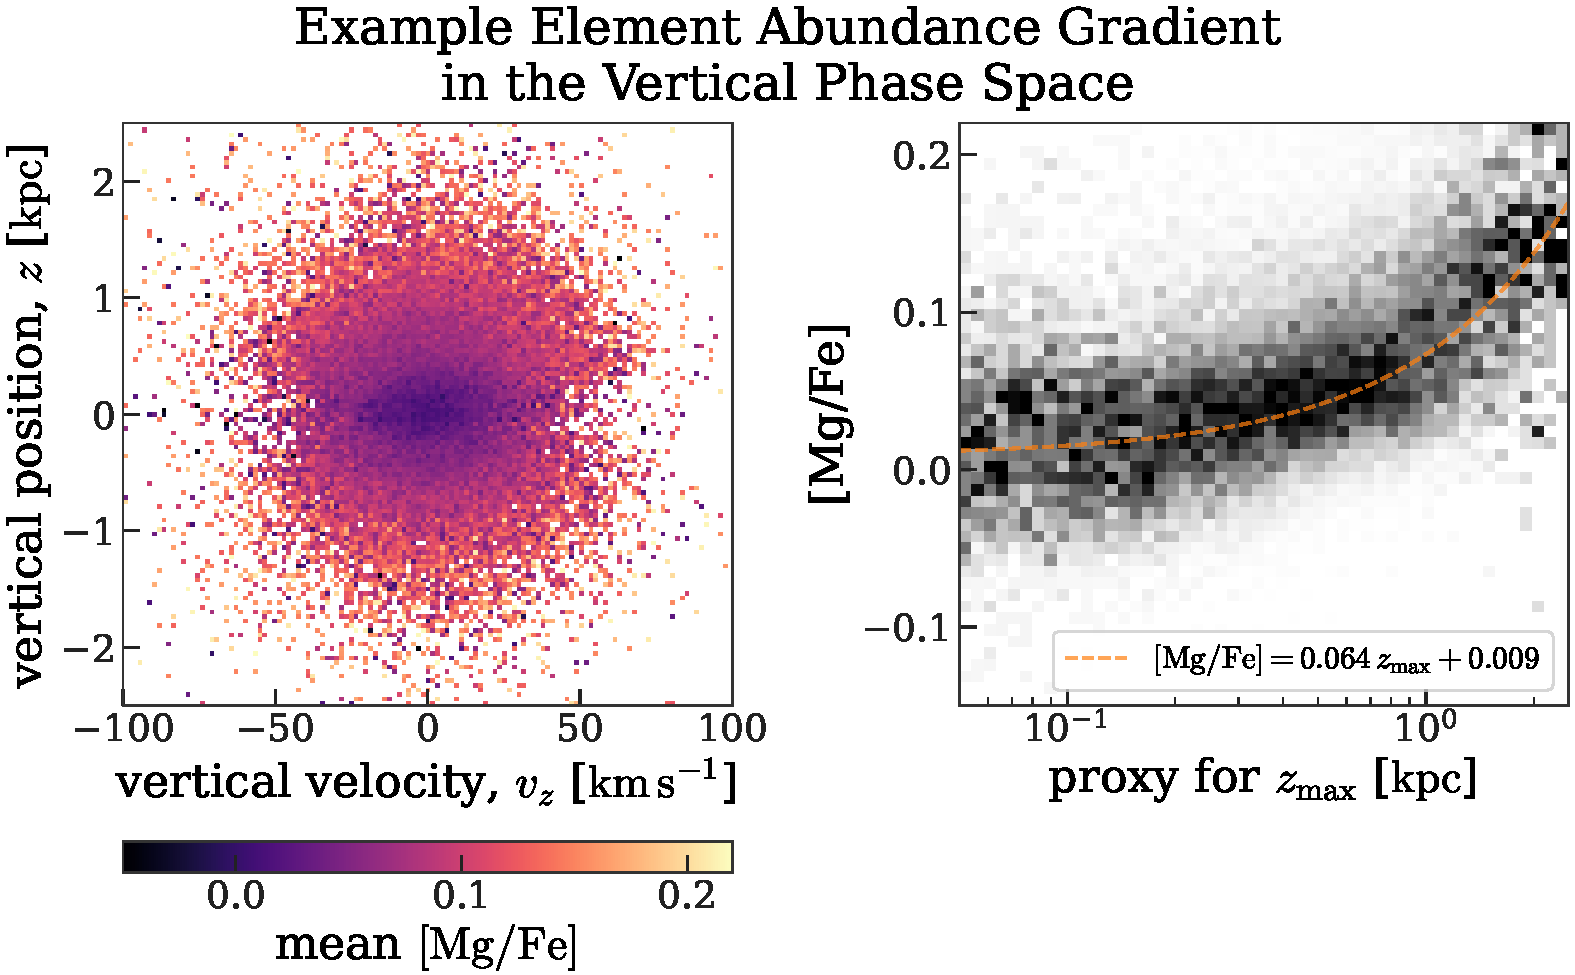
\includegraphics[width=1\textwidth]{mgfe-zvz.pdf}
\end{center}
\caption{%
A demonstration that stellar labels correlate with stellar orbits in the vertical phase
space of the Milky Way disk.
\textbf{Left panel:} Seven orbits computed in a Milky Way mass model (see
Appendix~\ref{sec:appendix-potential}) and shown in the vertical phase space, $(z,
v_z)$.
The orbits have equally-spaced values of the maximum height above the midplane each
orbit reaches, \zmax.
The vertical action, $J_z$, of these orbits scales approximately like $J_z \propto
\zmax^2$, and all orbits have $J_R=0$ and $J_\phi\approx 1900~\kms~\kpc$.
\textbf{Middle panel:} The mean \abun{Mg}{Fe} abundance for stars in the low-$\alpha$
sequence and with angular momenta $L_z$ within $\pm 15\%$ of the value for a circular
orbit at the Sun's position ($L_{z, c} \approx 1900$).
The mean \abun{Mg}{Fe} abundance is shown in small bins of the vertical position, $z$,
and velocity, $v_z$.
The mean abundance is systematically different for stars with low vertical action $J_z$
(i.e. near $(z, v_z) \sim (0, 0)$) as compared to stars with larger vertical action.
\label{fig:mgfe-zvz}
\textbf{Right panel:} The column-normalized density of stars in \abun{Mg}{Fe} as a
function of an observable proxy for the maximum height above the midplane reached by a
star, $\zmax$.
We estimate a proxy for \zmax\ without using a potential model by selecting only stars
with $|v_z| < 10~\kms$ (i.e. stars that are near their vertical apocenter).
The over-plotted dashed (orange) line shows a linear relation between \abun{Mg}{Fe} and
\zmax.
}
\end{figure*}


\section{Orbital Torus Imaging} \label{sec:oti}

The orbital actions $\bs{J}$ are useful quantities for summarizing orbits and
constructing dynamical models.
However, they require a global model for the gravitational potential, are expensive to
compute, and are not directly observable.
Fortunately, for increasingly large samples of stars in the Milky Way, we have access to
measurements of intrinsically-invariant stellar labels, such as surface element
abundance ratios or stellar ages.
These stellar labels can be used instead to trace out the orbit structure of the Galaxy.
This forms the basis of the method of Orbital Torus Imaging (OTI; CITE PW21), which we
describe below.
Here we build on past work (CITE PW21) by developing a new framework and implementation
of OTI that leverages modern auto-differentiation tools (e.g., \jax; \citealt{jax:2018})
to generalize and accelerate the model construction and fitting.


\subsection{Using stellar labels to map orbits}
\label{sec:oti-stat}

% TODO: mention "direct contouring" in phase-space density below -- and that the
% phase-space density itself can be a label

% From the shapes of these orbits, we can then infer the underlying acceleration field
% and therefore constrain the mass distribution of the Galaxy.
% We will also assume that, for each star, we have measurements of a set of invariant
% ``labels'' $\bs{F}$, and that those labels are correlated with the orbital properties
% of the tracers $\bs{F}(\bs{w})$, for now assuming the dependence is deterministic.

% In an equilibrium system where we have measured stellar kinematics $\bs{w} = (z, v_z)$
% and invariant labels $\bs{F}$ that appear to correlate with the orbits of stars, the
% labels can only depend on the phase-space coordinates through the vertical action
% $J_z$ or any function of the vertical action and not the vertical angle $\theta_z$.
% This comes from the assumption that the labels are invariant: If they depended on
% orbital angle $\theta_z$, this would imply that the labels change over the course of
% an orbit.

% We also then show how, with an OTI model of the orbit structure, this method can be used
% to compute empirical actions, angles, and frequencies that do not require assuming a
% global potential model.

Stars have a number of observable properties that are approximately invariant over their
lifetimes, or at least over galactic orbital timescales.
For example, the surface element abundance ratios, birth time (as a time-invariant proxy
of age), and stellar mass, to name a few.
We represent these quantities with the vector $\bs{Y}$, which we refer to as the
``stellar labels''.
In the Milky Way, these quantities are observed to correlate with the orbital
properties of stellar populations.
For example, there is a long known correlation between stellar age and velocity
dispersion (CITE), the kinematic properties of mono-abundance stellar populations depend
on the value of the abundance (CITE), and there are known gradients in stellar element
abundances and Galactic position (CITE).
Figure~\ref{fig:mgfe-zvz} shows an example of such a correlation in the vertical
kinematics of stars in the Milky Way.
The left panel of Figure~\ref{fig:mgfe-zvz} shows seven orbits in the vertical phase
space (with $J_R=0$ and $J_\phi \approx 1900~\kms~\kpc$), with equally-spaced values of
\zmax\ as computed in a Milky Way-like gravitational potential around the solar position
(see Section~\ref{sec:appendix-potential}).
The vertical action scales approximately with $J_z \propto \zmax^2$.
The middle panel shows the mean \abun{Mg}{Fe} abundance for stars in different locations
of the vertical phase space, demonstrating that stars with low-$J_z$ orbits (i.e. those
that stay near the center of this phase space) have systematically different element
abundances than stars with large-$J_z$ orbits (i.e. those that stay far from the center
of this phase space).


% The top left panel of Figure~\ref{fig:sim-contours} shows 8 orbits with different values
% of $J_z$ (but the same values of $J_R=0$ and a $J_\phi$ similar to the solar value)
% computed in a Milky Way-like gravitational potential (see
% Section~\ref{sec:appendix-potential}). \todo{define potential in appendix}
% The orbits are colored by their vertical action, demonstrating that orbits with larger
% vertical actions cover a larger area in vertical phase space and reach higher maximum
% heights above the midplane $z_{\textrm{max}}$.
% Note that the actions define surfaces that foliate the phase space; in the case of
% vertical dynamics, the 1D curves of constant $J_z$ (i.e. the orbits) can never
% intersect.

Under the assumptions we adopted in Section~\ref{sec:dynreview}, the correlations
between any intrinsic, time-invariant stellar properties $\bs{Y}$ and the orbital
properties of stars can only depend on the orbital actions $\bs{J}$ and not the angles
$\bs{\theta}$, which are time dependent.
This is useful because it means we can use the stellar labels as constants of motion
themselves to trace out the shapes of orbits in phase-space.
In the context of vertical dynamics, the vertical action $J_z$ is, by construction,
constant along an orbit, so any time-invariant function of the vertical action is also
constant along an orbit.

With a suitably large sample of stars, this provides a means to measure the orbital
structure the acceleration field of the Galaxy directly, without having to assume a form
for the potential and without needing to compute the actions.
As long as the gradient in stellar labels as a function of vertical action
$\deriv{Y}{J}$ is non-zero (i.e. not flat), we can use the level sets of constant
stellar label $Y$ to ``contour'' the orbits in the vertical phase space $(z,
v_z)$.\footnote{We note that this idea, in the context of using the phase-space density
as a stellar label, was briefly discussed in \citet{Kuijken:19XX} and referred to as
``direct contouring'' of the DF.}
From the orbit contours, we can directly measure the vertical acceleration $a_z$: For
any invariant stellar label $Y$, the total time derivative $\Deriv{Y}{t}$ must be equal
to zero,
\begin{align}
    \Deriv{Y}{t} &= \pderiv{Y}{t} +
        \pderiv{Y}{z} \, \deriv{z}{t} + \pderiv{Y}{v_z} \, \deriv{v_z}{t} = 0 \\
    0 &= \pderiv{Y}{z} \, v_z + \pderiv{Y}{v_z} \, a_z
\end{align}
where $a_z = \deriv{v_z}{t}$ is the vertical acceleration.
Rearranging this expression, we can write the vertical acceleration as
\begin{align}
    a_z &= - v_z \, \pderiv{Y}{z} \left(\pderiv{Y}{v_z}\right)^{-1} \label{eq:Y-az}
\end{align}
where the right hand side and partial derivatives are evaluated along a curve of
constant $Y$.

A simple example of this is the case where the stellar label $Y$ is a function of the
vertical energy $Y=Y(E_z)$ where
\begin{equation}
    E_z = \frac{1}{2} v_z^2 + \Phi_z(z)
\end{equation}
and $\Phi_z(z)$ is the vertical potential.
In this case, the partial derivatives in Equation~\ref{eq:Y-az} are:
\begin{align}
    \pderiv{Y}{z} &= \pderiv{Y}{E_z} \, \pderiv{\Phi_z}{z}\\
    \pderiv{Y}{v_z} &= \pderiv{Y}{E_z} \, v_z
\end{align}
so that
\begin{align}
    a_z &= - v_z \, \pderiv{\Phi_z}{z} \, \pderiv{Y}{E_z} \, \left(\pderiv{Y}{E_z} \, v_z\right)^{-1} \\
    a_z &= - \pderiv{\Phi_z}{z}
\end{align}
as expected.

Two subtleties complicate this idea.
For one, the labels are not deterministic functions of the actions.
For example, processes that cause dynamical heating of stars, which may introduce a
correlation between the vertical action, stellar age, and metallicity (CITE), are
inherently stochastic.
This means that, in general, for any value of the vertical action $J_z$, there will be
a distribution of possible stellar label values.
A second complication is that we only have a finite sample of stars, so we will
never observe two or more stars on \emph{exactly} the same orbit.
Together, these necessitate working with the distribution of stellar label values
conditioned on action, $p(\bs{Y} \given J_z(z, v_z))$, such that the distribution of
stellar label values has properties or parameters that vary smoothly with the vertical
action.

In the next section, we develop a method for fitting the contours of constant stellar
label that does not assume a form for the potential $\Phi_z(z_)$.
Instead of modeling the full distribution $p(\bs{Y} \given z, v_z)$, we assume that our
data are measurements of \emph{moments} of the distribution at different locations in
phase-space.
Contours of constant moments of the stellar label distribution equivalently satisfy the
expressions above (e.g., Equation~\ref{eq:Y-az}).
For example, the mean value of a stellar label $\mean{Y}$ is
\begin{equation}
    \mean{Y} = \int \dd Y \, Y \, p(Y \given J_z) \quad .
\end{equation}
It is straightforward to show that this also satisfies $\Deriv{\mean{Y}}{t} = 0$, along
with other moments of this distribution.


% - But: f(z, vz) = C define contours
%     - fit contours, can take derivatives
%     - Another benefit: contours are orbits, so can derive actions, angles, etc.
%     - Method called "direct contouring" by (KG paper 1)
% - <Explain our way of fitting shape of contours>

% The framework described in Section~\ref{sec:vertical} is a standard approach to modeling
% the vertical kinematics of tracers in the Milky Way disk to measure properties of the
% mass distribution, like the vertical acceleration or surface mass density.
% Here we describe an alternative approach, built off of the idea of Orbital Torus Imaging
% \citep[OTI;][]{Price-Whelan:2021}.
% OTI is the idea that, in an equilibrium system, any function of the phase-space
% coordinates that ``labels'' the orbits (e.g., the orbital actions or any function of
% the actions) can be used to constrain the shapes of contours of the DF.
% This is useful because the shapes of these contours are directly related to the
% acceleration (and therefore mass distribution) through the CBE
% (Equation~\ref{eq:cbe-1d}).
% In a system with one degree of freedom, these contours are closed curves in phase-space
% that also correspond to orbital trajectories.
% In what follows, we start by considering the case of using the phase-space density or
% the value of the DF itself to fit these contours.
% We then discuss how this generalizes to using stellar label data, which we assume are
% only functions of the orbital actions and not of orbital phase (i.e. conjugate angle).
% We finally show how, in the vertical phase-space, a fitted OTI model can be used to
% compute empirical values of dynamical quantities like the orbital actions, frequencies,
% and angles.

% A core motivation for OTI is that the derivatives of the DF that appear in the CBE
% (e.g., Equation~\ref{eq:cbe-1d}) only depend on the shapes of the curves defined by
% level sets of the DF (i.e. curves of constant phase-space density), or of any
% functions of the phase-space density that depend on auxiliary data (e.g., element
% abundance ratios or other stellar labels). In a system with one degree of freedom,
% these level sets are closed curves in phase-space that also correspond to orbits. We
% start by considering the case of using the phase-space density or the value of the DF
% itself, then discuss how this generalizes to using stellar label data, and then
% finally show how, in the vertical phase-space, a fitted OTI model can be used to
% compute empirical values of dynamical quantities like the orbital actions and
% frequencies.

\subsection{Modeling Stellar Label Moments that Correlate with Dynamics} \label{sec:}

\begin{figure*}[t!]
\begin{center}
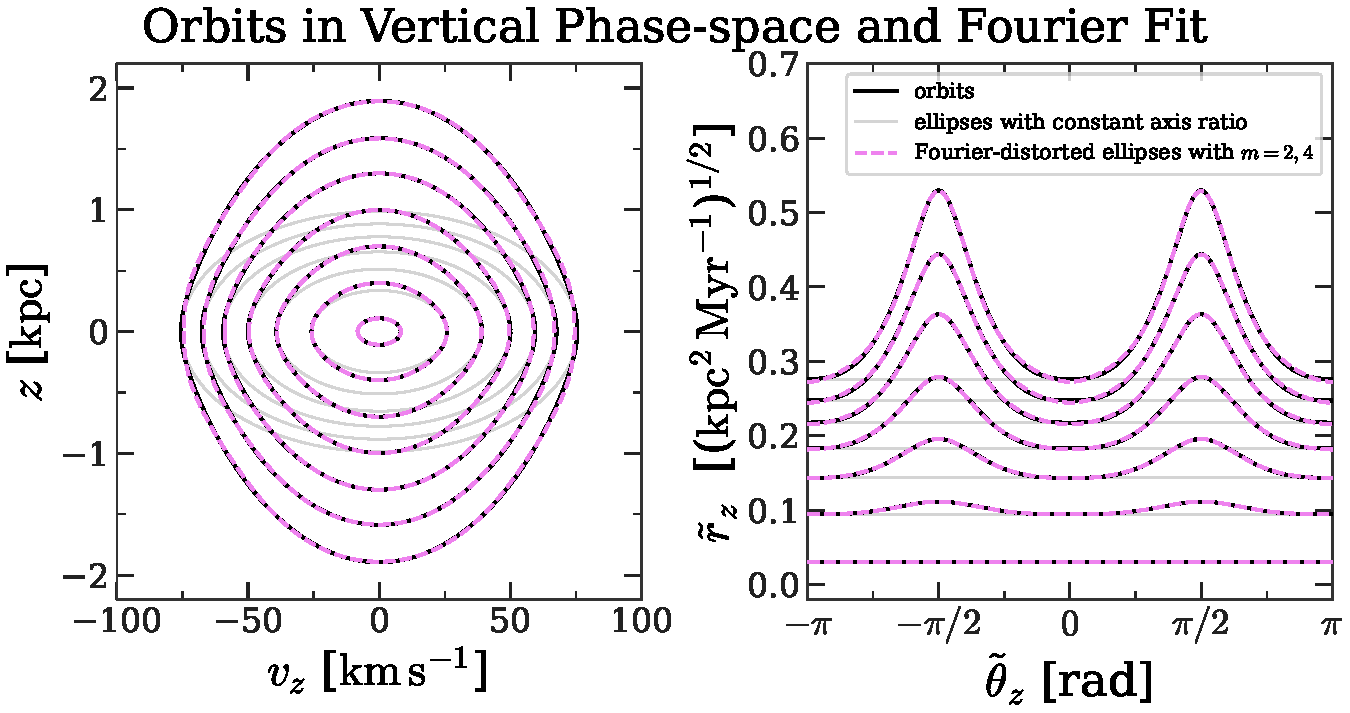
\includegraphics[width=\textwidth]{simulated-orbits-fourier.pdf}
\end{center}
\caption{%
TODO
\label{fig:fourier-contours}
}
\end{figure*}

In this section, we develop a method to fit the shapes of contours of constant stellar
label moments in the vertical phase space of the Milky Way disk.
An example of the type of data we would like to model is shown in the left panel of
Figure~\ref{fig:mgfe-zvz}.
As we showed in the previous section (Section~\ref{sec:oti-stat}), the shapes of these
contours correspond to the shapes of orbits in the vertical phase space (under the
assumptions listed above).
Figure~\ref{fig:XX} demonstrates this visually using simulated data.
We generate simulated stellar positions and velocities by sampling from a
quasi-isothermal distribution function (\df; CITE Binney, Sanders and Binney) embedded
in a static, axisymmetric model for the Milky Way.
The Milky Way potential model is described in Appendix~\ref{sec:appendix-potential}, and
we use the \agama\ package (CITE) to generate \todo{N} samples from the \df.
We then sub-select a sample of star particles that are spatially localized near the
solar radius, $|R - 8.3~\kpc| < 0.5~\kpc$, and are near their guiding radius, $|R - R_G|
< 0.5~\kpc$ where $R_G \equiv L_z / v_c(R)$ and $v_c(R)$ is the circular velocity at the
radius $R$.
We compute the maximum height above the midplane reached by each star particle, \zmax,
and use the linear relation between \zmax\ and \abun{Mg}{Fe} seen in the \apogee\ data
(see the right panel of Figure~\ref{fig:mgfe-zvz}) to compute simulated \abun{Mg}{Fe}
abundances for the star particles.
The leftmost panel of Figure~\ref{fig:XX} ...


That is, near the midplane, contours of the DF will correspond to curves of constant
elliptical radius \rzp, defined as
\begin{equation}
    \rzp = \sqrt{(z-z_0)^2 \, \freqzero + (v_z-v_{z,0})^2 \, \freqzero^{-1}} \label{eq:rzp}
\end{equation}
for all values of the corresponding ellipsoidal angle \thzp,
\begin{equation}
    \tan (\thzp) = \left(\frac{z-z_0}{v_z-v_{z,0}}\right) \, \freqzero
    \label{eq:thetazp}
\end{equation}
where $z_0$ and $v_{z,0}$ are the zero-point position and velocity, respectively, which
we include as parameters in our model.
Away from the midplane, the shapes of orbits have steadily decreasing frequencies with
increasing maximum height $z_{\textrm{max}}$, which leads to, to first order, a changing
aspect ratio of the contours.\todo{reference a figure panel?}
For contours with sufficiently large $z_{\textrm{max}}$ values (i.e. orbits that reach
many scale heights above the disk), the influence of the dark matter halo's potential
distorts the orbit shapes, and the contours of the DF are no longer well-approximated by
ellipses.\todo{a figure to show this point?}
The halo potential causes the orbits to deform from ellipses to more diamond-like shapes
that are reminiscent of $m=4$ Fourier modes.

To model more general contour shapes (i.e. beyond ellipses), we use a low-order Fourier
expansion in the ellipsoidal angle \thzp\ to distort the ellipsoidal radius \rzp\
into the distorted ellipsoidal radius \rz, defined as
\begin{equation}
    \rz = \rzp \, \left[1 + \sum_m \epsilon_m(\rzp) \, \cos{\left(m\,\thzp\right)}\right] \label{eq:rz}
\end{equation}
where, for the vertical kinematics, we only consider even $m$ values to preserve the
symmetry of the contour shapes.
The functions $\epsilon_m(\rzp)$ describe the radius-dependent amplitude of the Fourier
terms, which we require to all be zero at $\rzp=0$, and the values are typically $\ll
1$ within a few disk scale heights.
This expansion is motivated by the fact that we expect to need just a few Fourier terms:
an $m=2$ distortion with an amplitude that varies with \rzp\ will change the aspect
ratio of the elliptical contours as a function of \rzp, which acts like a changing
frequency as a function of $z_{\textrm{max}}$.
An $m=4$ distortion can ``pinch'' the contour shapes to make then more diamond-like,
which mimics the effect of an orbit feeling the halo potential.
In applications below, we try different maximum $m$ values, \mmax, beyond
$m=4$.
\todo{Could show plots of rzp vs thetazp with different Fourier mmax fits?}

The distorted radius \rz\ (Equation~\ref{eq:rz}) is effectively a label for the orbits
and therefore also labels contours of the DF.
To fit the phase-space density with the distorted radius \rz, we then need to specify
a functional form for the dependence of the phase-space density on \rz, $f_z(\rz)$.

The model components that must be specified in order to fit the phase-space density
distribution of a sample of stellar phase-space positions are then: the Fourier
distortion amplitude functions $\epsilon_m(\rzp)$ for all $m$ orders up to the specified
\mmax, the functional form of the phase-space density $f_z(\rz)$, and the
zero-point position and velocity $z_0$ and $v_{z,0}$.
We have implemented this framework in \python\ using \jax\ \citep{jax:2018} to
accelerate the model evaluation and to use automatic differentiation to compute the
gradients of the model with respect to the (many) model parameters.
This framework is therefore very general and accepts any functional forms for the model
components.
We discuss specific choices for these components in the applications below
(Sections~\ref{sec:applications-sim} and \ref{sec:applications-data}).

From a fitted model, we can compute the vertical acceleration at any $(z, v_z)$ ...


\subsection{Modeling Stellar Label} \label{sec:stellarlabels}

TODO: Jeans theorem: any function of the actions / integrals of motion gives a steady-state solution of the CBE.


\subsection{Estimating Dynamical Quantities} \label{sec:todo}

Given an orbital trajectory in the vertical phase-space, and after fitting a model to
the DF (Section~\ref{sec:psd}) or stellar label distribution
(Section~\ref{sec:stellarlabels}), we can estimate dynamical quantities like the orbital
actions, angles, and frequencies without needing to assume a form for the gravitational
potential.
In terms of the vertical position and velocity $z, v_z$, if we are given a function
$v_z(z)$ along an orbit, we can compute the vertical action $J_z$ and vertical period
$T_z$ as
\begin{align}
    J_z &= 4 \times \frac{1}{2\,\pi} \, \int_0^{z_{\textrm{max}}} \dd z \, v_z(z) \\
    T_z &= 4 \times \int_0^{z_{\textrm{max}}} \frac{\dd z}{v_z(z)}\quad ,
\end{align}
from which the vertical frequency follows, $\Omega_z = \frac{2\pi}{T_z}$.
For a given instantaneous position and velocity $z^*, v_z^*$, the vertical angle
\thz\ at that point can be computed as the fraction of an orbital period traversed
up to that point,
\begin{equation}
    \thz = \frac{2\pi}{T_z} \, \int_0^{z} \frac{\dd z'}{v_z(z' \,;\, \rz(z^*, v_z^*))} \quad ,
\end{equation}
where $z'$ is an integration variable, and the function $v_z(z' \,;\, \rz(z^*, v_z^*))$
indicates that this is a curve at constant \rz\ as determined by the model parameters
and given phase-space position $(z^*, v_z^*)$.

In principle, if we could observe the stellar tracer DF with infinite particle
resolution, we could extract contours of constant density (or stellar labels) to
numerically and directly estimate the integrals described above.
This would obviate the need for the modeling framework described in the previous two
subsections (Sections~\ref{sec:psd}--\ref{sec:stellarlabels}).
Of course, in practice, we are limited by the finite number of stars in our sample so
that this procedure would be noisy and unstable in regions of low phase-space density,
which are often the most interesting (e.g., the transition from disk-dominated to
halo-dominated kinematics where dark matter dominates the gravitational potential).
Instead, the framework described above allows us to fit a smooth model to the tracer data and to use this to semi-empirically estimate the dynamical quantities of interest.




\subsection{Estimating Dynamical Quantities from the Phase-space Density}

Given a distribution of $N$ stellar positions and velocities $\{z, v_z\}_N$, our task is
to infer the parameters of a functional model for the number density $n(z, v_z)$ that
also allows use to compute the dynamical quantities ($J_z$, $\Omega_z$, $\theta_z$) for
any individual $z, v_z$.
With our assumption that the \df\ is phase-mixed, the number density should only depend
on the phase-space coordinates through the action, so that $n(z, v_z) = n(J_z(z, v_z))$
At fixed $z$, say $z=0$, we expect that $J_z$ increases with increasing $v_z$ (orbits
with larger velocity at the midplane will reach larger heights) and $\Omega_z$
decreases with increasing $v_z$ (orbits that reach larger heights above the midplane
have longer periods).
Similar arguments can be made at fixed $v_z=0$ in considering how $J_z$ and $\Omega_z$
vary with increasing $z$.
It is therefore useful to construct an ellipsoidal polar coordinate system in the $z,
v_z$ plane with a radius coordinate \rzp\ and a corresponding angle coordinates
$\theta_z'$ defined as
\begin{align}
    \rzp &= \sqrt{z^2 \, \omega_0 + v_z^2 \, \omega_0^{-1}} \label{eq:rzp} \\
    \theta_z' &= \tan^{-1}\left(\frac{z}{v_z}\,\omega_0\right) \label{eq:thetazp}
\end{align}
where $\omega_0$ is a scale frequency.
The vertical action $J_z$ and frequency $\Omega_z$ should be close to monotonic
functions of this polar radius $r_z'$.

For example, in a simple harmonic oscillator (SHO) potential,
\begin{equation}
    \Phi(z) = \frac{1}{2} \, \omega^2 \, z^2
\end{equation}
the Hamiltonian (total energy per unit mass) is
\begin{equation}
    H(z, v_z) = E_z = \frac{1}{2} \, v_z^2 + \frac{1}{2} \, \omega^2 \,z^2
\end{equation}
and the orbital action $J_z$ is given by
\begin{equation}
    J_z = \frac{E_z}{\omega} \quad .
\end{equation}
All orbits have the same frequency $\omega$ and are elliptical in the 1D phase-space.
In this case, the scale frequency $\omega_0$ in $r_z'$ corresponds to the frequency of
the oscillator $\omega_0=\omega$, the radius $r_z'$ is related to the action $J_z$ as
\begin{equation}
    J_z = \frac{1}{2} r_z'^2
\end{equation}
and the conjugate angle $\theta_z$ (conjugate to the action $J_z$) is equal to the
ellipsoidal angle $\theta_z = \theta_z'$.
The phase-mixed \df\ $f(J_z)$ can therefore be expressed as some
function of the polar radius alone $f(J_z)=g(r_z')$.

Orbits in even simple galactic mass models are more complex.
For example, in a two-component mass model consisting of a Galactic disk embedded in a
dark matter halo, the morphology of an orbit will depend on whether it is confined to
the disk or whether it feels the transition from the disk- to the halo-dominated region
of the mass distribution.
Figure~\ref{fig:zvz} (left panel) is an illustration that shows several sample orbits
with different values of the vertical action (spaced uniformly in $\sqrt{J_z}$), all
with $J_R=0$ and the same $J_\phi$ in a two-component galaxy model consisting of a
Miyamoyo--Nagai disk component \citep{Miyamoto:1975} and a Navarro--Frenk--White (NFW)
halo component \citep{NFW:1996}.
For this toy galaxy model, parameters are chosen to roughly match the local circular
velocity and scale height of the Milky Way disk, but this potential model is only used
for illustrative purposes (the parameter values are not important).
For smaller values of the vertical action, orbits are close to elliptical in shape.
Moving out in ``radius'' or vertical action $J_z$, orbits have frequencies that decrease
with increasing action (which manifests as a changing axis ratio of the orbits).
For orbits with larger vertical action (i.e. orbits that reach scale heights more than a
few times the adopted scale height $h_z=0.25~\kpc$), the orbits begin to significantly
feel the influence of the dark matter halo and the orbital trajectory shapes become more
``pinched'' or ``diamond''-like near $z=0$.
We expect these features to be generic for slices of the vertical kinematics in galaxies
like the Milky Way: The vertical frequency should be a smooth function of the vertical
action, and orbits will have more complex morphologies (i.e. more complex than
ellipses).

Whereas in a SHO potential the orbital trajectories are functionally equivalent
(ellipses) and scaled by the value of the action, in a more generic galactic mass model
we expect the trajectories to distort away from ellipses.
As we saw in Figure~\ref{fig:zvz}, this distortion changes the orbital frequency of
orbits with increased size or vertical action (i.e., changes the scale frequency of the
ellipse), but also introduces a morphological change by making the orbits more
diamond-shaped, especially close to $z=0$.
In terms of action--angle coordinates, this means that the ellipsoidal angle introduced
above (Equation~\ref{eq:thetazp}) is no longer equal to the conjugate angle $\theta_z$,
and any functional model for the phase-mixed \df\ $f(J)$ must be a function of both the
ellipsoidal radius and angle:
\begin{equation}
    f(J) = g(r_z', \theta_z') \quad .
\end{equation}
We choose to express this density model as a function of an auxiliary variable $r_z$
that is defined as a low-order Fourier expansion distortion to the ellipsoidal radius
$r_z'$:
\begin{align}
    r_z &= r_z' \, \left[1 + \sum_m \epsilon_m(r_z') \, \cos{\left(m\,\theta_z'\right)}\right] \label{eq:rz} \\
    n(z, v_z) &= n(r_z(r_z', \theta_z'))
\end{align}
where $n(\cdot)$ represents a density function and $\epsilon_m(r_z')$ represents a
distortion amplitude, whose magnitude is hopefully must smaller than one for all
relevant values of $r_z'$ --- that is, we assume that
\begin{equation}
    |\epsilon_m(r_z')| \ll 1 \,\, \forall r_z', m \quad .
\end{equation}

With this parametrization, the action and frequency are monotonic and smooth functions
of the distorted radius $r_z$: $J_z = J_z(r_z)$ and $\Omega_z = \Omega_z(r_z)$.
We can also now compute the dynamical quantities with integrals over the ellipsoidal
angle $\theta_z'$
\begin{align}
    J_z(r_z) &= \frac{2}{\pi} \, \int_0^{\pi/2} \dd \theta_z' \, v_z(\theta_z')
        \, \left|\frac{\dd z}{\dd \theta_z'}\right| \\
    T_z &= 4 \, \int_0^{\pi/2} \frac{\dd \theta_z'}{v_z(\theta_z')}
        \, \left|\frac{\dd z}{\dd \theta_z'}\right|
\end{align}
where
\begin{align}
    v_z(\theta_z') &= \sqrt{\omega_0} \, r_z'(r_z, \theta_z') \, \cos{(\theta_z')} \\
    z(\theta_z') &= \frac{1}{\sqrt{\omega_0}} \, r_z'(r_z, \theta_z') \, \sin{(\theta_z')}
\end{align}
and $r_z'(r_z, \theta_z')$ in general has to be found by numerical root-finding of
Equation~\ref{eq:rz}.


\subsection{Orbital Torus Imaging with Stellar Labels} \label{sec:oti-labels}
Like previous subsection, but $F(r_z)$ instead of $f(r_z)$
- But wait, there's more!
- Functions of f also satisfy CBE, so we can contour anything that has a gradient with dynamics!
- For example, moments of element abundances
- Advantage: Easier to measure from data and less subject to selection effects
- Show how


\section{Applications to Simulated Data} \label{sec:applications-sim}

In what follows, we demonstrate the OTI framework described above using a set of
simulated datasets of increasing complexity.
We start by using a one-dimensional simple harmonic oscillator potential
(Section~\ref{sec:sim-sho}), then use a more realistic multi-component galaxy model
(Section~\ref{sec:sim-eq}), and finally use the final snapshot from an $N$-body
simulation of a disk galaxy perturbed by an orbiting satellite
(Section~\ref{sec:sim-jason}).

% For our implementation used in this article, we adopt the following:
% \begin{align}
%     m &= \left\{2, 4\right\} \\
%     e_2(r_z') &\geq 0 \,\,\forall r_z'\\
%     e_4(r_z') &\leq 0 \,\,\forall r_z'
% \end{align}
% and we use linear splines to represent the functions $n(r_z)$, $e_2(r_z')$, and
% $e_4(r_z')$.

\subsection{Simple Harmonic Oscillator}
\label{sec:sim-sho}

As an initial application, we simulate phase-space data in a harmonic oscillator
potential,
\begin{equation}
    \Phi_{z}(z) = \frac{1}{2} \, \omega^2 \, z^2
\end{equation}
by sampling from an isothermal distribution function\footnote{We will use $f(\cdot)$ to
represent a \df\ that integrates to a number of stars, and $p(\cdot)$ to represent a
normalized \df\ that integrates to 1 (i.e. a probability distribution function).}
\begin{align}
    p_z(J_z) &= \frac{1}{\, s_z} e^{-\frac{J_z}{s_z}} \quad ; \quad J_z \in [0, \infty)\\
    s_z &= \sigma_{v_z}^2 / \omega\\
    z = \sqrt{\frac{2 \, J_z}{\omega}} \, \sin\theta_z \quad &; \quad
        v_z = \sqrt{2 \, J_z \, \omega} \, \cos\theta_z
\end{align}
We adopt $\omega = 0.08~\unit{\radian\per\mega\year}$ and $s_z = 50~\kms$ as arbitrary
choices meant to approximately match the observed vertical kinematics of stars near the
solar position (CITE e.g.,).
We sample $N=2^{18}=\num{262144}$ phase-space positions as another arbitrary choice, but note that
the precision of our measurements (especially at high $z$) will depend on the sample
size.
Figure~\ref{fig:sho-data-model} (left panel) shows the log-number density of this
simulated sample in the vertical phase-space.
We will first fit the phase-space density of the simulated stars, hoping to recover a
constant frequency for all orbits and a vertical acceleration close to $a_z(z) =
-\omega^2\,z$.
For setting axis limits and functions below, we define a maximum elliptical radius
$r_{z, \textrm{max}} = 5 \, \frac{s_z}{\sqrt{\omega}}$ equivalent to the $5~\sigma$
values of the \df\ scale.
In terms of the phase-space coordinates, we then use a maximum $z$ value of $\max(z) =
r_{z, \textrm{max}} \times \sqrt{\omega}$ and similarly for $v_z$, $\max(v_z) = r_{z,
\textrm{max}} / \sqrt{\omega}$.
For the choices above, this corresponds to $\max(z) \approx 3~\kpc$ and $\max(v_z)
\approx 250~\kms$.

\begin{figure*}[t!]
\begin{center}
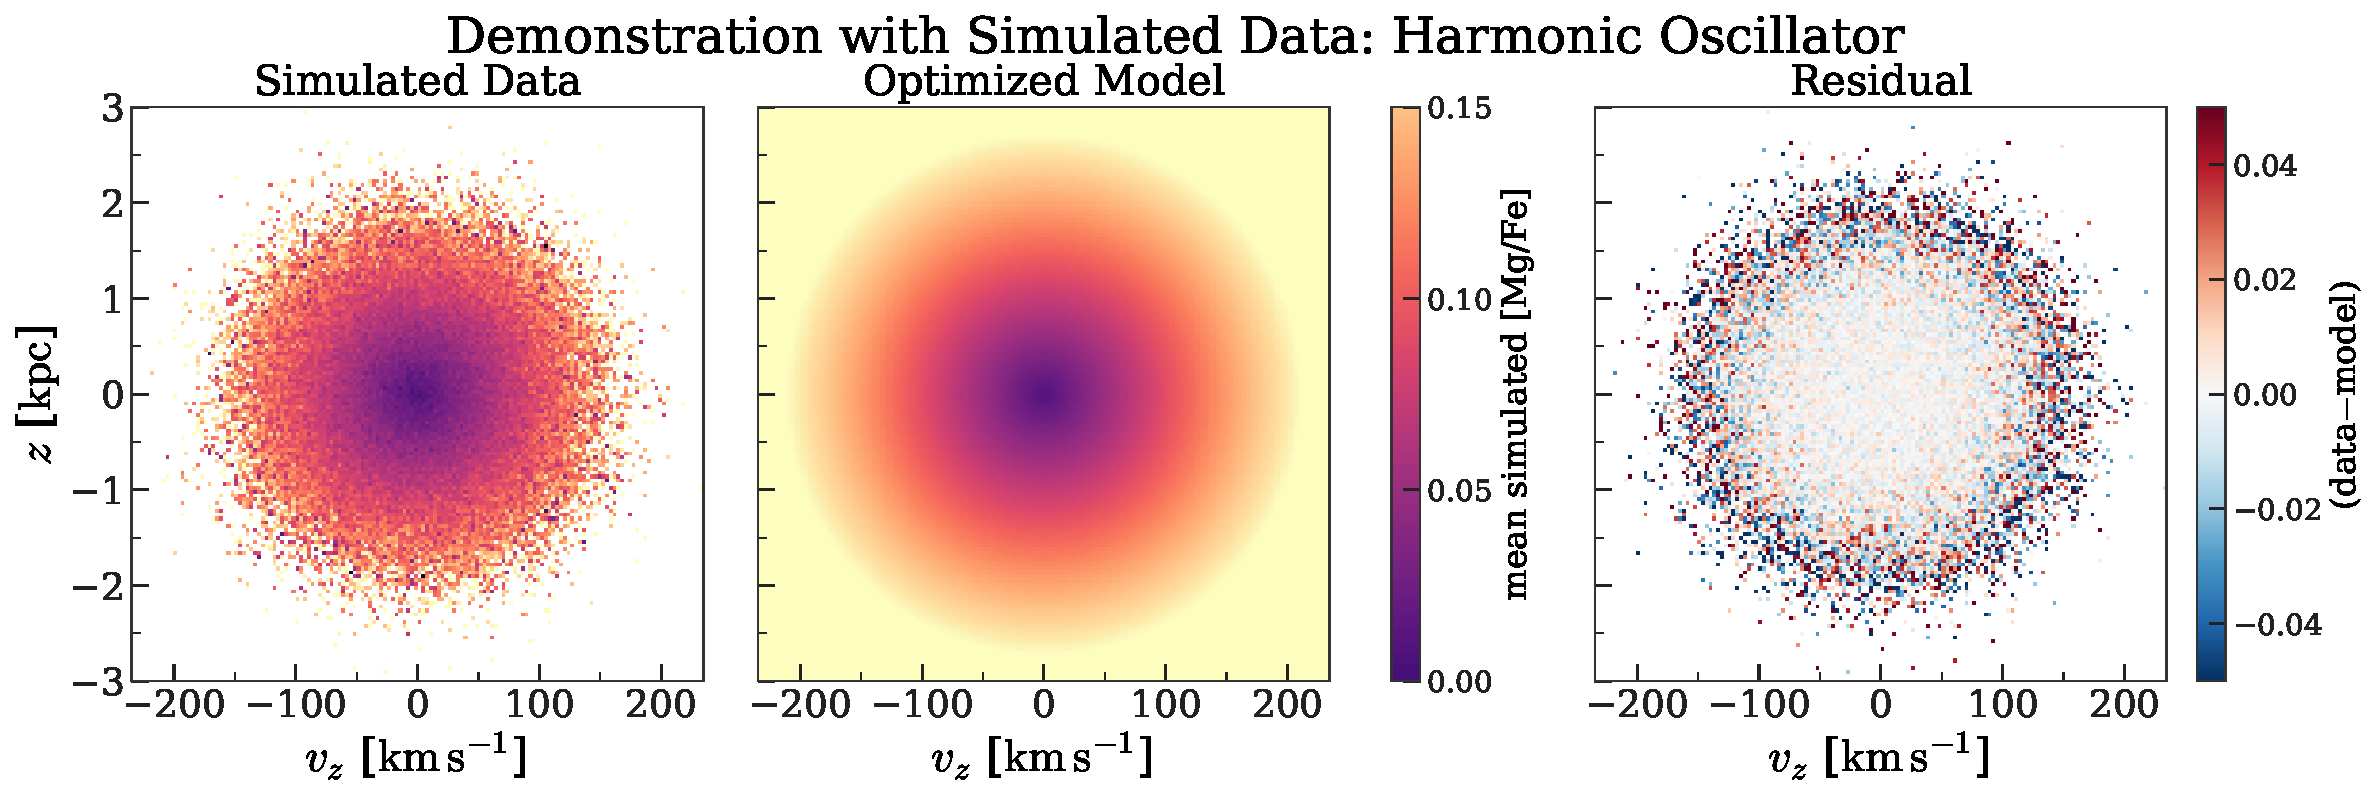
\includegraphics[width=\textwidth]{sho-data-model.pdf}
\end{center}
\caption{%
TODO
\label{fig:sho-data-model}
}
\end{figure*}

We then need to decide on functional forms for both the log-density function,
$\ln\left(n(\rz)\right)$, and the Fourier coefficient function, $e_2(\rzp)$.
For each, we use a monotonic quadratic spline function defined such that the function is
always monotonically increasing or decreasing (which must be hard-set before
optimization).
\todo{Describe monotonic quadratic spline in appendix}
For the log-density function, we assert that the log-density must monotonically
decrease from $\rz = 0$ to the maximum spline knot location.
We use 10 spline knot locations $x_k^{(\ln n)}$ equally spaced in $\rz$ between $0$ and
$r_{z, \textrm{max}}$.

For this initial case, we include only an $m=2$ term in our Fourier distortion of the
elliptical radius (Equation~\ref{eq:rz}).
For the Fourier coefficient function, we require that the coefficient value must equal
zero at $\rzp = 0$, i.e. $e_2(0) = 0$, and that the coefficient value monotonically
increases with $\rzp$.
Requiring $e_2(0) = 0$ ensures that the parameter $\freqzero$ corresponds to the
asymptotic orbital frequency as $\rzp \rightarrow 0$.
Assuming that the coefficient value increases with $\rzp$ (so that the orbit shapes
can only become more prolate with increasing $z_{\textrm{max}}$) is equivalent to
assuming that the volume density increases with increasing height $z$.
We use 5 spline knot locations $x_k^{(e_2)}$ equally spaced in $\rz$ between $0$ and
$r_{z, \textrm{max}}$, but we require the knot value at $\rzp = 0$ to be equal to zero
$y_0^{(e_2)}=0$.

All of the parameters used in this demonstrative model fit are summarized in
Table~\ref{tbl:sho-params}.

\begin{table}
    \begin{centering}
\begin{tabular}{c c c}
    \multicolumn{3}{c}{\textbf{Simple Harmonic Oscillator Model Fit}} \\ [0.75ex]
    Parameter & Description & Bounds \\ [0.5ex]
    \hline\hline
    $\ln(\freqzero / (\unit{\radian\per\mega\year}))$ & Asymptotic frequency at $r_z=0$ & $(-9, 0)$\\
    $z_0$ & Solar position relative to midplane & $(-0.5, 0.5)~\kpc$\\
    $v_{z,0}$ & Solar velocity relative to midplane & $(-50, 50)~\kms$\\
    $y_0^{\ln n}$ & Log-phase-space density function value at $r_z=0$ & $(-5, 25)$\\
    $y_{1\dots K}^{\ln n}$ & Log-phase-space density function derivative values & $(-25, 0)$\\
    $y_0^{e_2}$ & $m=2$ Fourier coefficient function value at $r_z=0$ & fixed to $0$\\
    $y_{1\dots L}^{e_2}$ & $m=2$ Fourier coefficient function derivative values & $(0, 1)$\\
\end{tabular}
\caption{
    A summary of the parameters and parameter bounds used for fitting the simulated
    simple harmonic oscillator data in Section~\ref{sec:sim-sho}.
    We use $K=10$ spline knots for the log-phase-space density spline function and $L=5$
    spline knots for the $m=2$ Fourier coefficient spline function.
    In total, this model has 17 free parameters.
    \label{tbl:sho-params}
}
\end{centering}
\end{table}

\subsection{Simple Equilibrium Model}
\label{sec:sim-eq}

Set up an Agama model, show that we can recover the acceleration field.


\subsection{N-body Simulation with a Perturbed Disk}
\label{sec:sim-jason}


\section{Applications to Data} \label{sec:applications-data}

\subsection{Mapping ... spirals ... \gaia\ Data Release 3}
\label{sec:gaiadr3}

TODO: Empirical actions - show frequency-theta with empirical

Fit the vertical acceleration in a slice around the sun, ignoring selection function.
Show residuals: Phase spiral-o-rama


\subsection{Empirical Actions and Frequencies}
\label{sec:gaiadr3}

TODO: compare Agama with empaf


\subsection{GALAH or APOGEE demonstration}
\label{sec:gaiadr3}


\section{Discussion} \label{sec:discussion}

\subsection{Limitation that our acceleration can depend on $v_z$}


\section{Summary and Conclusions} \label{sec:conclusions}


\begin{acknowledgements}

It is a pleasure to thank ...

% Funding for the Sloan Digital Sky Survey IV has been provided by the Alfred P.
% Sloan Foundation, the U.S. Department of Energy Office of Science, and the
% Participating Institutions. SDSS-IV acknowledges support and resources from the
% Center for High-Performance Computing at the University of Utah. The SDSS web
% site is www.sdss.org.

% SDSS-IV is managed by the Astrophysical Research Consortium for the
% Participating Institutions of the SDSS Collaboration including the Brazilian
% Participation Group, the Carnegie Institution for Science, Carnegie Mellon
% University, the Chilean Participation Group, the French Participation Group,
% Harvard-Smithsonian Center for Astrophysics, Instituto de Astrof\'isica de
% Canarias, The Johns Hopkins University, Kavli Institute for the Physics and
% Mathematics of the Universe (IPMU) / University of Tokyo, Lawrence Berkeley
% National Laboratory, Leibniz Institut f\"ur Astrophysik Potsdam (AIP),
% Max-Planck-Institut f\"ur Astronomie (MPIA Heidelberg), Max-Planck-Institut
% f\"ur Astrophysik (MPA Garching), Max-Planck-Institut f\"ur Extraterrestrische
% Physik (MPE), National Astronomical Observatories of China, New Mexico State
% University, New York University, University of Notre Dame, Observat\'ario
% Nacional / MCTI, The Ohio State University, Pennsylvania State University,
% Shanghai Astronomical Observatory, United Kingdom Participation Group,
% Universidad Nacional Aut\'onoma de M\'exico, University of Arizona, University
% of Colorado Boulder, University of Oxford, University of Portsmouth, University
% of Utah, University of Virginia, University of Washington, University of
% Wisconsin, Vanderbilt University, and Yale University.

This work has made use of data from the European Space Agency (ESA) mission
{\it Gaia} (\url{https://www.cosmos.esa.int/gaia}), processed by the {\it Gaia}
Data Processing and Analysis Consortium (DPAC,
\url{https://www.cosmos.esa.int/web/gaia/dpac/consortium}). Funding for the DPAC
has been provided by national institutions, in particular the institutions
participating in the {\it Gaia} Multilateral Agreement.

\end{acknowledgements}

\software{
    Astropy \citep{astropy:2013, astropy:2018, astropy:2022},
    gala \citep{gala},
    IPython \citep{ipython},
    numpy \citep{numpy},
    % pymc3 \citep{Salvatier2016},
    % schwimmbad \citep{schwimmbad:2017},
    scipy \citep{scipy}.
}

\appendix

\section{A Toy Milky Way Mass Model}
\label{sec:appendix-potential}

TODO.

\section{Evaluation of the Vertical Acceleration from an OTI Model}
\label{sec:appendix-math}

We would like to evaluate the vertical acceleration as a function of height above the
Galactic midplane, $a_z(z) = \frac{\partial \Phi}{\partial z}$.
From the collisionless Boltzmann equation (Equation~\ref{eq:cbe-1d}), after rearranging
terms, we have:
\begin{align}
    \frac{\partial \Phi}{\partial z} &=
        v_z \, \frac{\partial f}{\partial z} \,
        \left( \frac{\partial f}{\partial v_z} \right)^{-1} \\
    &= v_z \, \frac{\partial f}{\partial \rz} \, \frac{\partial \rz}{\partial z} \,
        \left( \frac{\partial f}{\partial \rz} \frac{\partial \rz}{\partial v_z} \right)^{-1} \\
        &= v_z \, \frac{\partial \rz}{\partial z} \,
        \left( \frac{\partial \rz}{\partial v_z} \right)^{-1}
\end{align}
The acceleration only depends on the shapes of the contours of the DF, i.e. curves of
constant \rz, so that we only need to differentiate the distorted radius to evaluate it.
Recall that, based on our definitions above,
\begin{align}
    \rzp &= \sqrt{z^2 \, \freqzero + v_z^2 \, \freqzero^{-1}} \\
    \thzp &= \tan^{-1}\left(\frac{z}{v_z} \, \freqzero\right) \\
    \rz &= \rzp \, \left( 1 + \sum_{m=2}^{\mmax} e_m(\rzp) \,
        \cos(m \, \thzp) \right) \label{eq:rz-rzp}
\end{align}
where the sum in Equation~\ref{eq:rz-rzp} is only over even values of $m$.

We must compute the partial derivatives of \rz\ with respect to $z$ and $v_z$:
\begin{align}
    \frac{\partial \rz}{\partial z} &=
        \frac{\partial \rzp}{\partial z} +
        \sum_{m=2}^{\mmax} \frac{\partial}{\partial z} \left[\rzp \, e_m(\rzp) \, \cos\left(m \, \thzp\right)\right]\\
    \frac{\partial \rz}{\partial v_z} &=
        \frac{\partial \rzp}{\partial v_z} +
        \sum_{m=2}^{\mmax} \frac{\partial}{\partial v_z} \left[\rzp \, e_m(\rzp) \, \cos\left(m \, \thzp\right)\right]
\end{align}

To work out the resulting expressions, we will make use of the following terms:
\begin{alignat}{3}
    \frac{\partial \rzp}{\partial z} &= \frac{z\,\freqzero}{\rzp} \quad &; \quad
        \frac{\partial \rzp}{\partial v_z} &= \frac{v_z}{\freqzero \, \rzp} \\
    \frac{\partial \thzp}{\partial z} &= \frac{v_z}{\rzp^2} \quad &; \quad
        \frac{\partial \thzp}{\partial v_z} &= -\frac{z}{\rzp^2} \\
    \frac{\partial e_m}{\partial z} &=
        \frac{\partial e_m}{\partial \rzp} \, \frac{\partial \rzp}{\partial z}
        \quad &; \quad
        \frac{\partial e_m}{\partial v_z} &=
        \frac{\partial e_m}{\partial \rzp} \, \frac{\partial \rzp}{\partial v_z}
\end{alignat}

Our goal is to remove or collect terms that explicitly contain $v_z$, as we are going to
take the limit as $\thzp \to \frac{\pi}{2}$, i.e. to evaluate the acceleration along the
$z$-axis, which implies $v_z \to 0$.
Starting with the derivative with respect to $z$:
\begin{align}
    \frac{\partial \rz}{\partial z} &=
        \frac{\partial \rzp}{\partial z} +
        \sum_{m=2}^{\mmax} \frac{\partial}{\partial z}
            \left[\rzp \, e_m(\rzp) \, \cos(m \, \thzp)\right]\\
    &= \frac{\partial \rzp}{\partial z} +
        \sum_{m=2}^{\mmax} \left[
        \frac{\partial \rzp}{\partial z} \, e_m \, \cos(m \, \thzp)
        + \rzp \, \frac{\partial e_m}{\partial z} \, \cos(m \, \thzp)
        - \rzp \, e_m \, \sin(m \, \thzp) \, m \,\frac{\partial \thzp}{\partial z}\right]\\
    &= \frac{z\,\freqzero}{\rzp} + \sum_{m=2}^{\mmax} \left[
        \frac{z\,\freqzero}{\rzp} \, e_m \, \cos(m \, \thzp) +
        \rzp \, \frac{z\,\freqzero}{\rzp} \, \frac{\partial e_m}{\partial \rzp} \, \cos(m \, \thzp) -
        \rzp \, e_m \, \sin(m \, \thzp) \, m \, \frac{v_z}{\rzp^2}\right]\\
    &= \frac{z\,\freqzero}{\rzp} \, \left[
        1 + \sum_{m=2}^{\mmax} \left(
            e_m \, \cos(m \, \thzp) +
                \rzp \, \frac{\partial e_m}{\partial \rzp} \, \cos(m \, \thzp) -
                m \, e_m \, \sin(m \, \thzp) \, \frac{v_z}{z\,\freqzero}
        \right)
    \right]\\
    &= \frac{z\,\freqzero}{\rzp} \, \left[
        1 + \sum_{m=2}^{\mmax} \left(
            \left(e_m + \rzp \, \frac{\partial e_m}{\partial \rzp}\right) \,
                \cos(m \, \thzp) -
            m \, e_m \, \frac{\sin(m \, \thzp)}{\sin(\thzp)} \, \cos(\thzp)
        \right)
    \right]
\end{align}
As we are interested in evaluating this expression along the $z$-axis, we will take the
limit of this expression as $\thzp \to \frac{\pi}{2}$.
For even values of $m$, as we require, the sine term in the sum will be zero, and the
cosine terms become:
\begin{equation}
    \cos(m \, \thzp) = (-1)^{m/2} \quad .
\end{equation}
In this limit, the expression becomes:
\begin{equation}
    \lim_{\thzp \to \frac{\pi}{2}} \frac{\partial \rz}{\partial z} =
        \frac{z\,\freqzero}{\rzp} \, \left[
            1 + \sum_{m=2}^{\mmax} (-1)^{m/2} \,
                \left(e_m + \rzp \, \frac{\partial e_m}{\partial \rzp}\right)
        \right] \quad .
\end{equation}

Similarly for the derivative with respect to $v_z$:
\begin{align}
    \frac{\partial \rz}{\partial v_z} &=
        \frac{\partial \rzp}{\partial v_z} +
        \sum_{m=2}^{\mmax} \frac{\partial}{\partial v_z}
            \left[\rzp \, e_m(\rzp) \, \cos(m \, \thzp)\right]\\
    &= \frac{\partial \rzp}{\partial v_z} +
        \sum_{m=2}^{\mmax} \left[
        \frac{\partial \rzp}{\partial v_z} \, e_m \, \cos(m \, \thzp)
        + \rzp \, \frac{\partial e_m}{\partial v_z} \, \cos(m \, \thzp)
        - \rzp \, e_m \, \sin(m \, \thzp) \, m \,\frac{\partial \thzp}{\partial v_z}\right]\\
    &= \frac{v_z}{\freqzero\,\rzp} + \sum_{m=2}^{\mmax} \left[
        \frac{v_z}{\freqzero\,\rzp} \, e_m \, \cos(m \, \thzp) +
        \rzp \, \frac{v_z}{\freqzero\,\rzp} \, \frac{\partial e_m}{\partial \rzp} \, \cos(m \, \thzp) +
        \rzp \, e_m \, \sin(m \, \thzp) \, m \, \frac{z}{\rzp^2}\right]\\
    &= \frac{v_z}{\freqzero \, \rzp} \, \left[
        1 + \sum_{m=2}^{\mmax} \left(
            e_m \, \cos(m \, \thzp) +
                \rzp \, \frac{\partial e_m}{\partial \rzp} \, \cos(m \, \thzp) +
                m \, e_m \, \sin(m \, \thzp) \, \tan(\thzp)
        \right)
    \right]\\
    &= \frac{v_z}{\freqzero \, \rzp} \, \left[
        1 + \sum_{m=2}^{\mmax} \left(
            \left(e_m + \rzp \, \frac{\partial e_m}{\partial \rzp}\right) \,
                \cos(m \, \thzp) +
            m \, e_m \, \sin(m \, \thzp) \, \tan(\thzp)
        \right)
    \right]
\end{align}
Taking the same limit $\thzp \to \frac{\pi}{2}$, this expression becomes:
\begin{equation}
    \lim_{\thzp \to \frac{\pi}{2}} \frac{\partial \rz}{\partial v_z} =
        \frac{v_z}{\freqzero \, \rzp} \, \left[
            1 + \sum_{m=2}^{\mmax} (-1)^{m/2} \,
                \left(e_m\,(1 - m^2) + \rzp \, \frac{\partial e_m}{\partial \rzp}\right)
        \right] \quad .
\end{equation}

Combining these expressions, we have:
\begin{align}
    \frac{\partial \Phi}{\partial z} &=
        v_z \, \frac{\partial \rz}{\partial z} \,
        \left( \frac{\partial \rz}{\partial v_z} \right)^{-1}\\
    &= v_z \, \frac{z\,\freqzero}{\rzp} \, \frac{\freqzero \, \rzp}{v_z} \,
        \frac{\left[
            1 + \sum_{m=2}^{\mmax} (-1)^{m/2} \,
                \left(e_m + \rzp \, \frac{\partial e_m}{\partial \rzp}\right)
        \right]}{\left[
            1 + \sum_{m=2}^{\mmax} (-1)^{m/2} \,
                \left(e_m\,(1 - m^2) + \rzp \, \frac{\partial e_m}{\partial \rzp}\right)
        \right]} \\
    &= \freqzero^2 \, z \,
        \frac{\left[
            1 + \sum_{m=2}^{\mmax} (-1)^{m/2} \,
                \left(e_m + \rzp \, \frac{\partial e_m}{\partial \rzp}\right)
        \right]}{\left[
            1 + \sum_{m=2}^{\mmax} (-1)^{m/2} \,
                \left(e_m\,(1 - m^2) + \rzp \, \frac{\partial e_m}{\partial \rzp}\right)
        \right]}
\end{align}

\bibliographystyle{aasjournal}
\bibliography{refs}

\end{document}
